\documentclass[a4paper,12pt]{book}

\usepackage{simple_booklet_style}

\usepackage{blindtext}

\definecolor{bannercolor}{rgb}{0.3922,0.5843,0.9294}
\definecolor{nicered}{rgb}{.647,.129,.149}

\linespread{1.2} % make lines less crowded

\begin{document}

%----------------------------------------------------------------------------------------
%	TITLE PAGE
%----------------------------------------------------------------------------------------
    \title{Clustering the interstellar medium}

    \begingroup
    \thispagestyle{empty}
	\AddToShipoutPicture*{\put(0,0){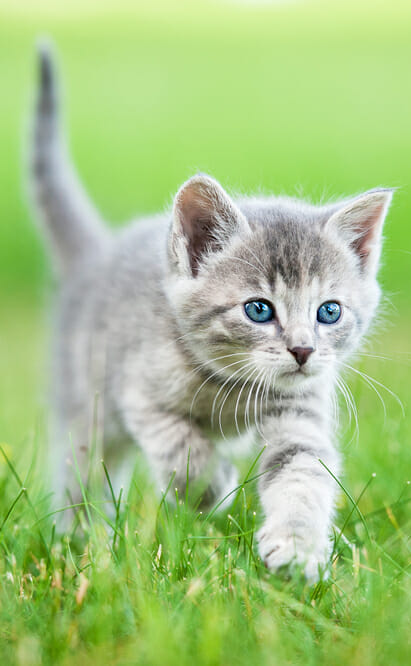
\includegraphics[scale=3]{cat1}}} % Image background

    \vspace*{9.75cm} % height above strip
	\hspace*{-3.5cm} % left starting for strip
	%\put(0 mm, 142 mm) % copied from https://www.overleaf.com/latex/templates/matnat-compendium/xbfgbfgzpcxz
	%{ % Given a picture, we overlay a banner, rather than modifying the picture itself
		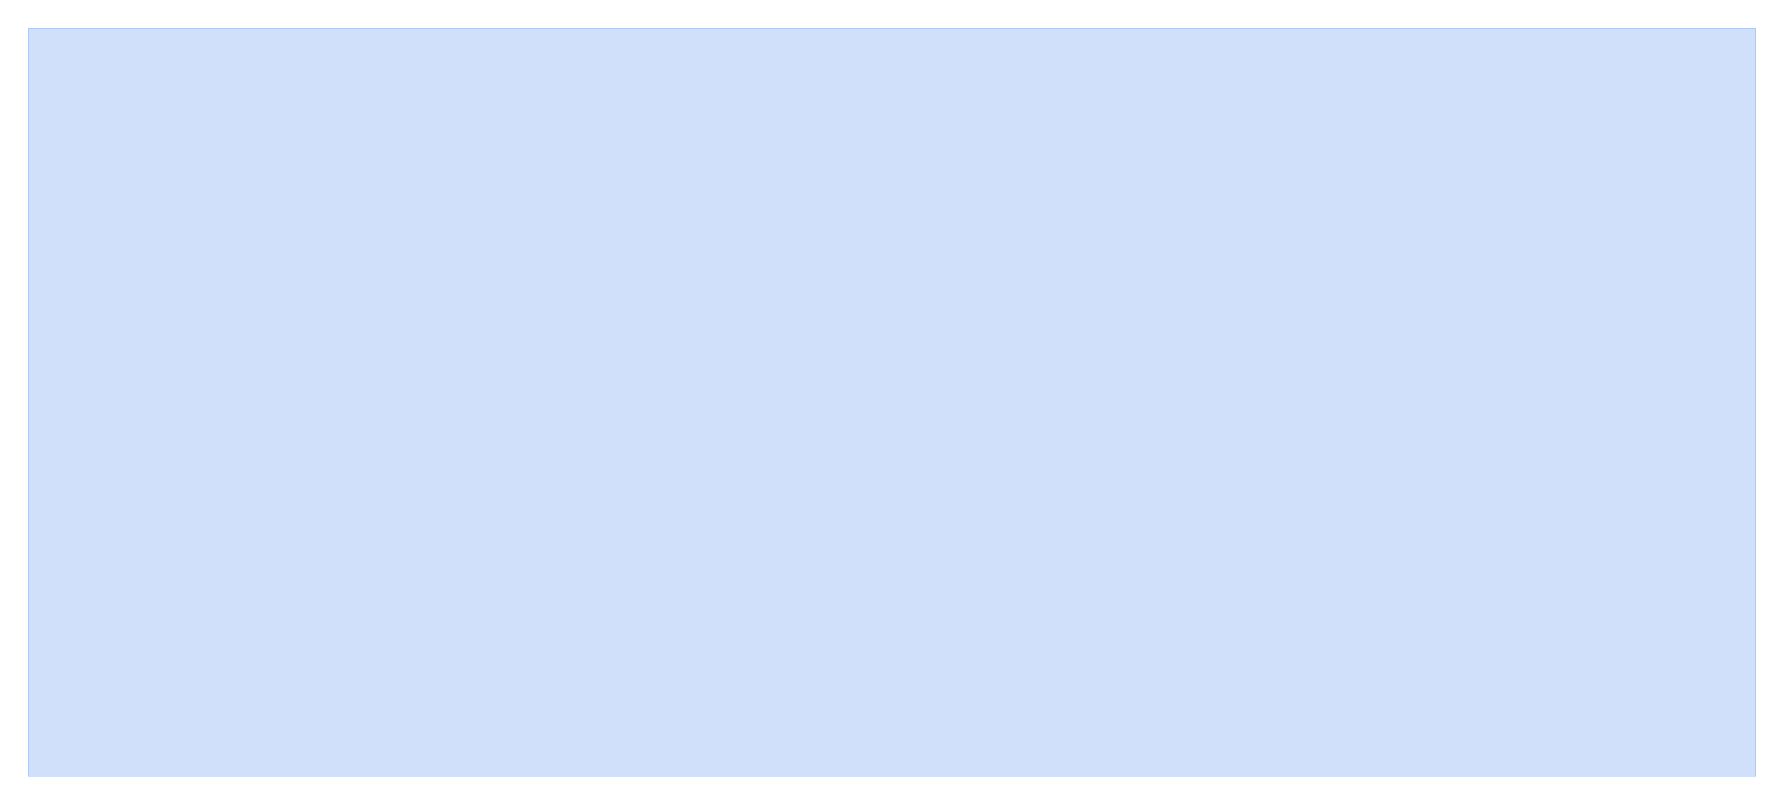
\begin{tikzpicture}%[scale = 1mm]
			\filldraw[bannercolor, opacity = 0.3]
			(0, 0) rectangle (\paperwidth + 10, 9.5); % length and width of strip
		\end{tikzpicture}
	%}
	\centering
	\vspace*{-9cm} % go back to the top of strip to write
	\par\normalfont\fontsize{35}{35}\sffamily\selectfont
	\textbf{Do Cats Always Land on Their Feet?}\\
	{\LARGE That's how they have 9 lives!}\par % Book title
	\vspace*{1cm}
	{\Huge Flying Cats}\par % Author name
    \endgroup

%----------------------------------------------------------------------------------------
%	COPYRIGHT PAGE
%----------------------------------------------------------------------------------------
    \newpage
    \thispagestyle{empty}
    ~\vfill

    \noindent Copyright \copyright\ 2021 John Smith % Copyright notice

    \noindent \textsl{Published by Publisher} % Publisher

    \noindent \textit{book-website.com} % URL

    \noindent Licensed under the Creative Commons Attribution-NonCommercial 3.0 Unported License
    (the ``License'').
    You may not use this file except in compliance with the License.
    You may obtain a copy of the License at \url{https://creativecommons.org/licenses/by-nc/3.0}.
    Unless required by applicable law or agreed to in writing, software distributed under the
    License is distributed on an \textsc{``as is'' basis, without warranties or conditions of any
    kind}, either express or implied.
    See the License for the specific language governing permissions and limitations under the
    License. % License information, replace this with your own license (if any)

    \noindent \textit{First printing, March 2021} % Printing/edition date

%----------------------------------------------------------------------------------------
%	TABLE OF CONTENTS
%----------------------------------------------------------------------------------------
    \pagestyle{empty} % Disable headers and footers for the following pages

    \tableofcontents % Print the table of contents itself

    % Forces the first chapter to start on an odd page so it's on the right side of the book
    %\cleardoublepage % not working
    \let\cleardoublepage\clearpage  % don't do this for paper books


%----------------------------------------------------------------------------------------
%	Chapters
%----------------------------------------------------------------------------------------
    \pagestyle{fancy} % Enable headers and footers again

    
\chapter{Introduction}
\minitoc

This is an introduction.

\section{Environment Setup}

This is a husky.

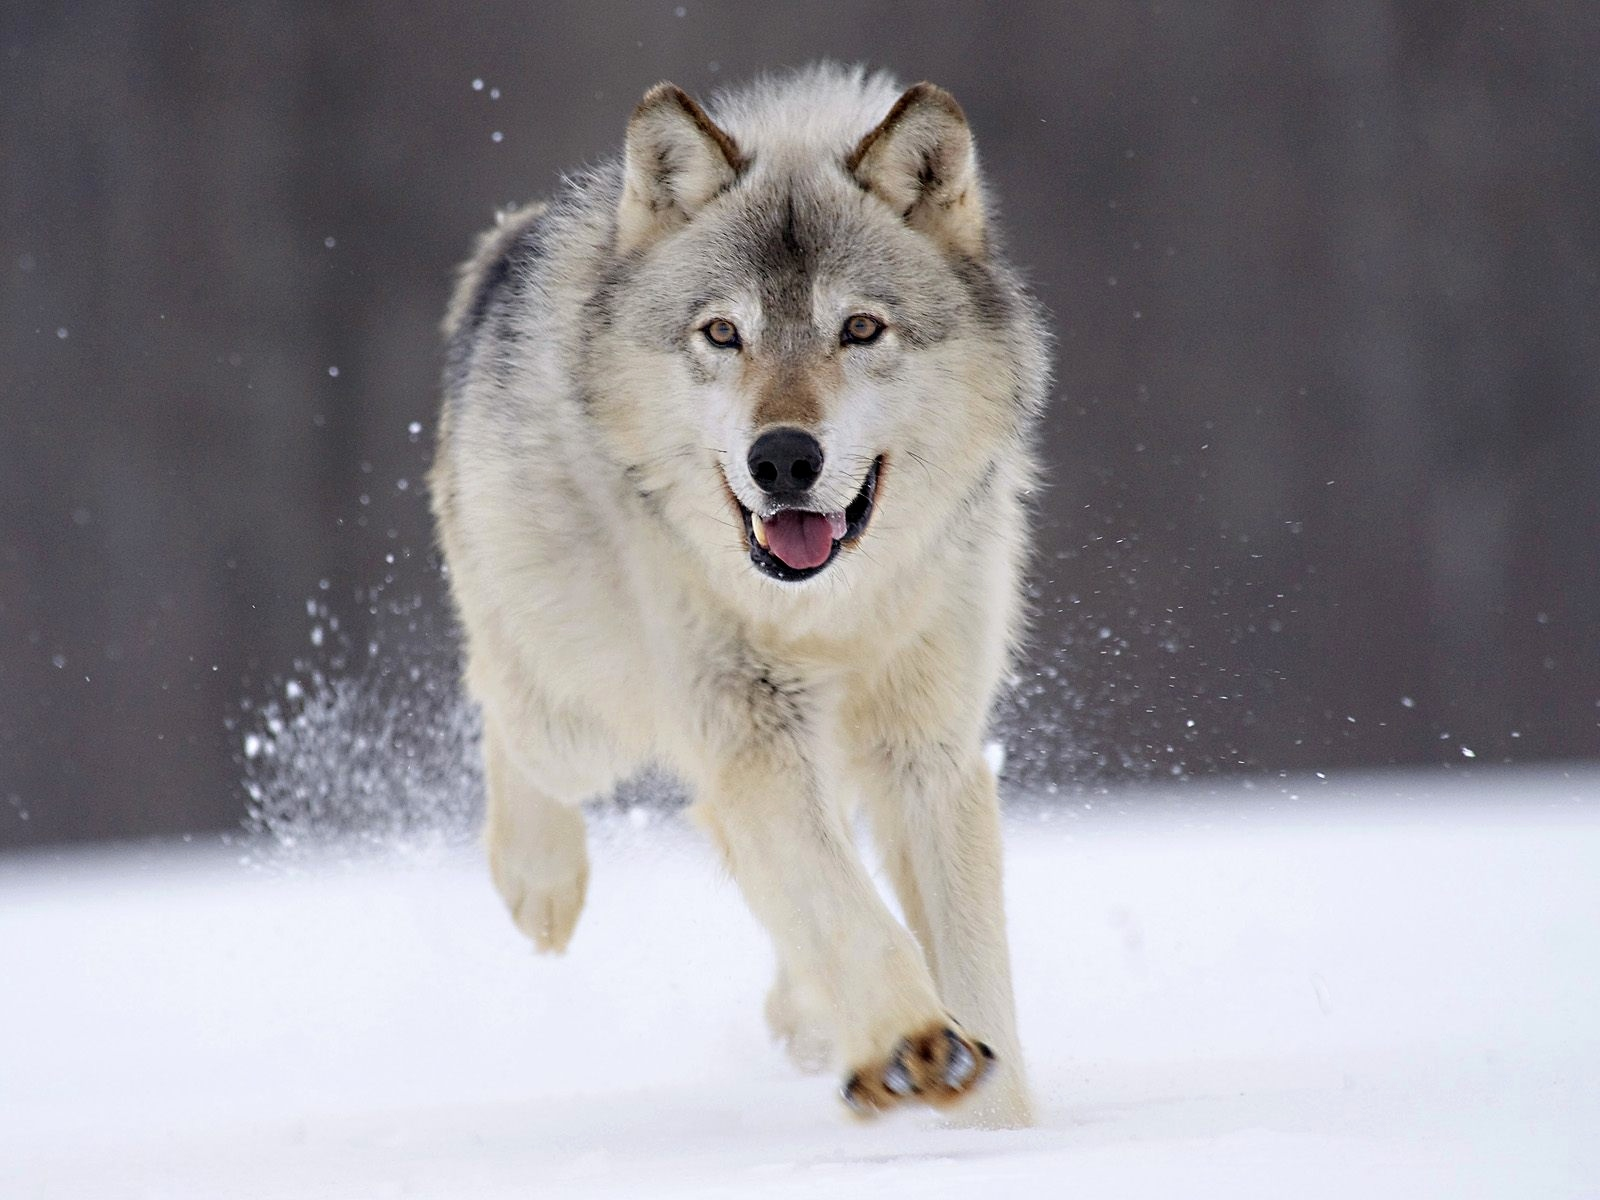
\includegraphics[scale=0.25]{chapter1/husky}

\blindtext[3]

\section{Get work done}

\blindtext[3]


    

\chapter{Deep Dive}
\minitoc

It's time to get more detailed facts.

\section{Environment Setup}

This is a treasure, 汗血宝马.

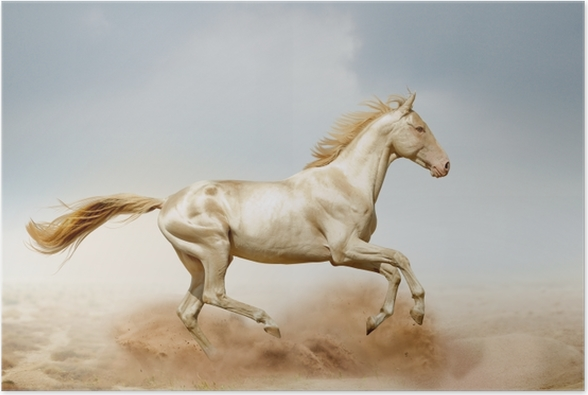
\includegraphics[scale=3]{chapter2/akhal_teke_horse}

\blindtext[3]

\section{Get work done}

\blindtext[3]

\section{Get work done}

\blindtext[3]


\end{document}
